%
% Sección de resultados de compraciones de desempeño.
% Artículo sobre tokenización.
%
% Proyecto Lovelace.
%

% TODO: pasar esto a GNUPlot.

\section{Resultados y conclusiones}
\label{sec:conclusiones}

\begin{table}
  \renewcommand{\arraystretch}{1.3}
  \centering
  \caption{Comparación de tiempos de tokenización.}
  \label{tabla:tiempos_tokenizacion}
  \begin{tabular}{c c c}
    \hline
     & Tokenización ($\mu$s) & Detokenización ($\mu$s) \\
    \hline
    FFX & 83 & 64 \\\hline 
BPS & 247 & 127 \\\hline 
TKR & 46260 & 373 \\\hline 
AHR & 3427 & 390 \\\hline 
DRBG & 54060 & 387 \\\hline 

    \hline
  \end{tabular}
\end{table}

\begin{figure*}[!t]
  \centering
  \subfloat[Tokenización y detokenización]{
    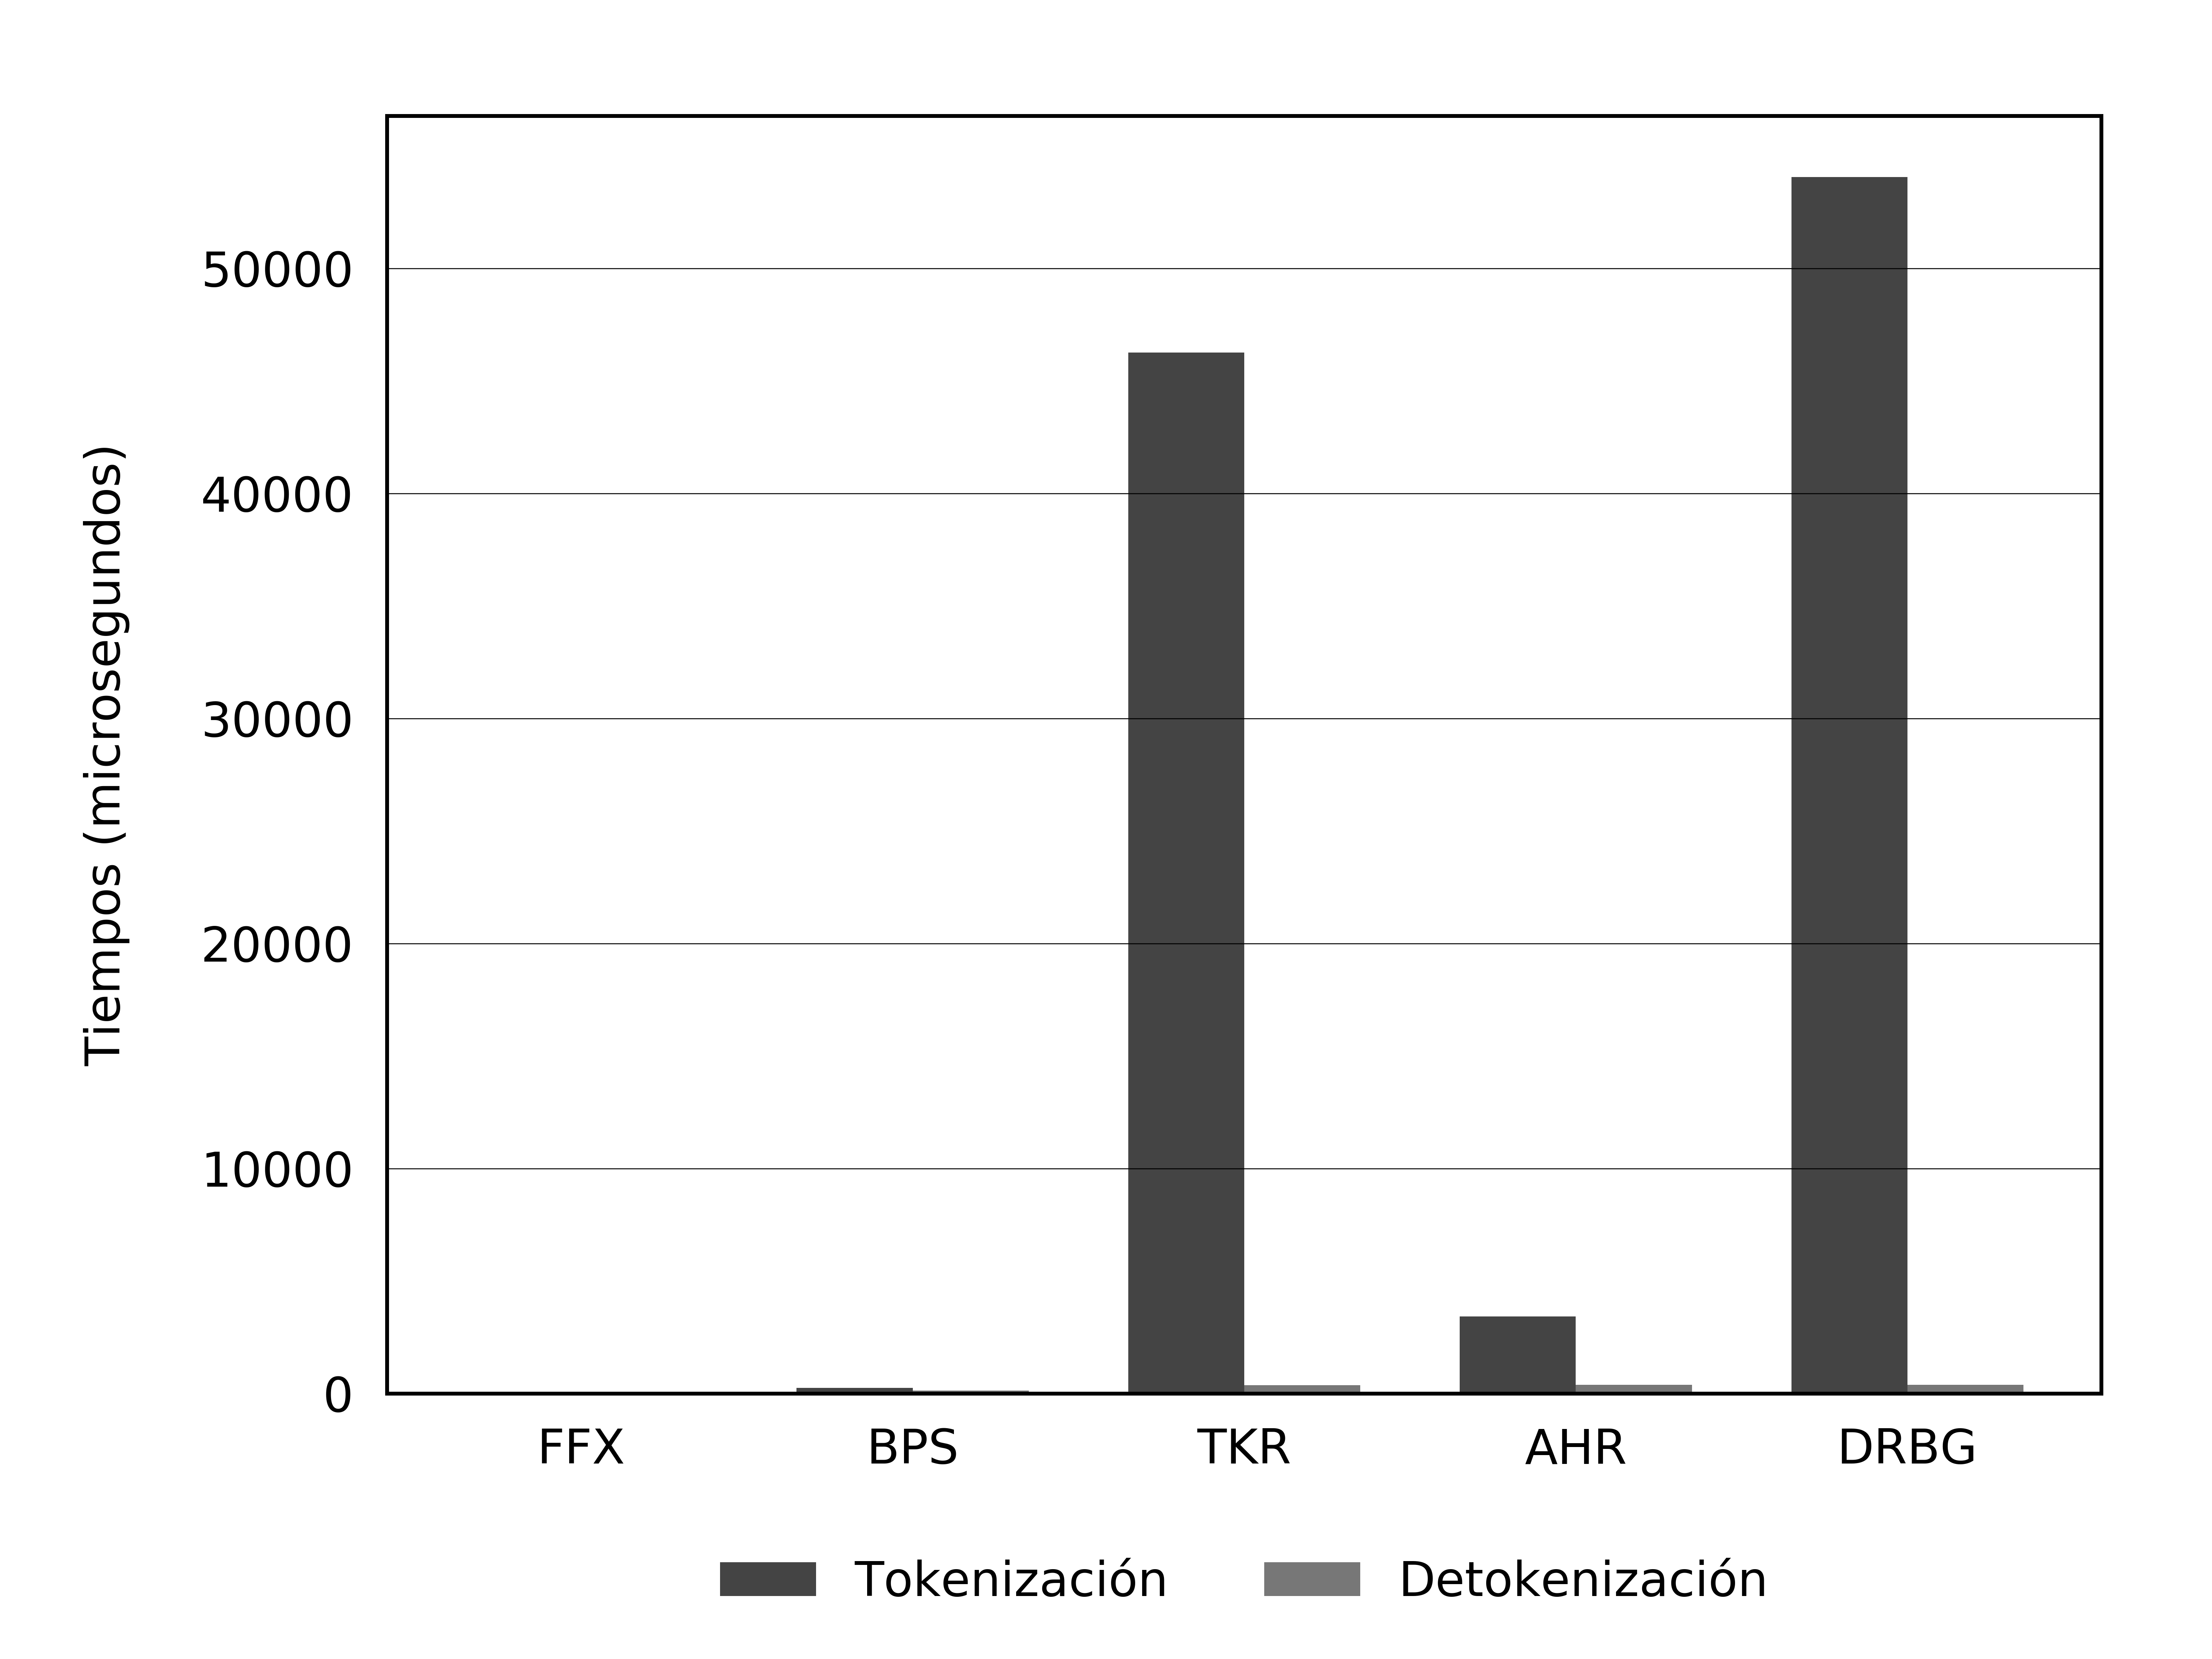
\includegraphics[width=0.5\linewidth]
      {../implementaciones/reportes/tiempos_unitarios.png}
    \label{figura:tiempos_unitarios}
  }
  \subfloat[Generación de tokens]{
    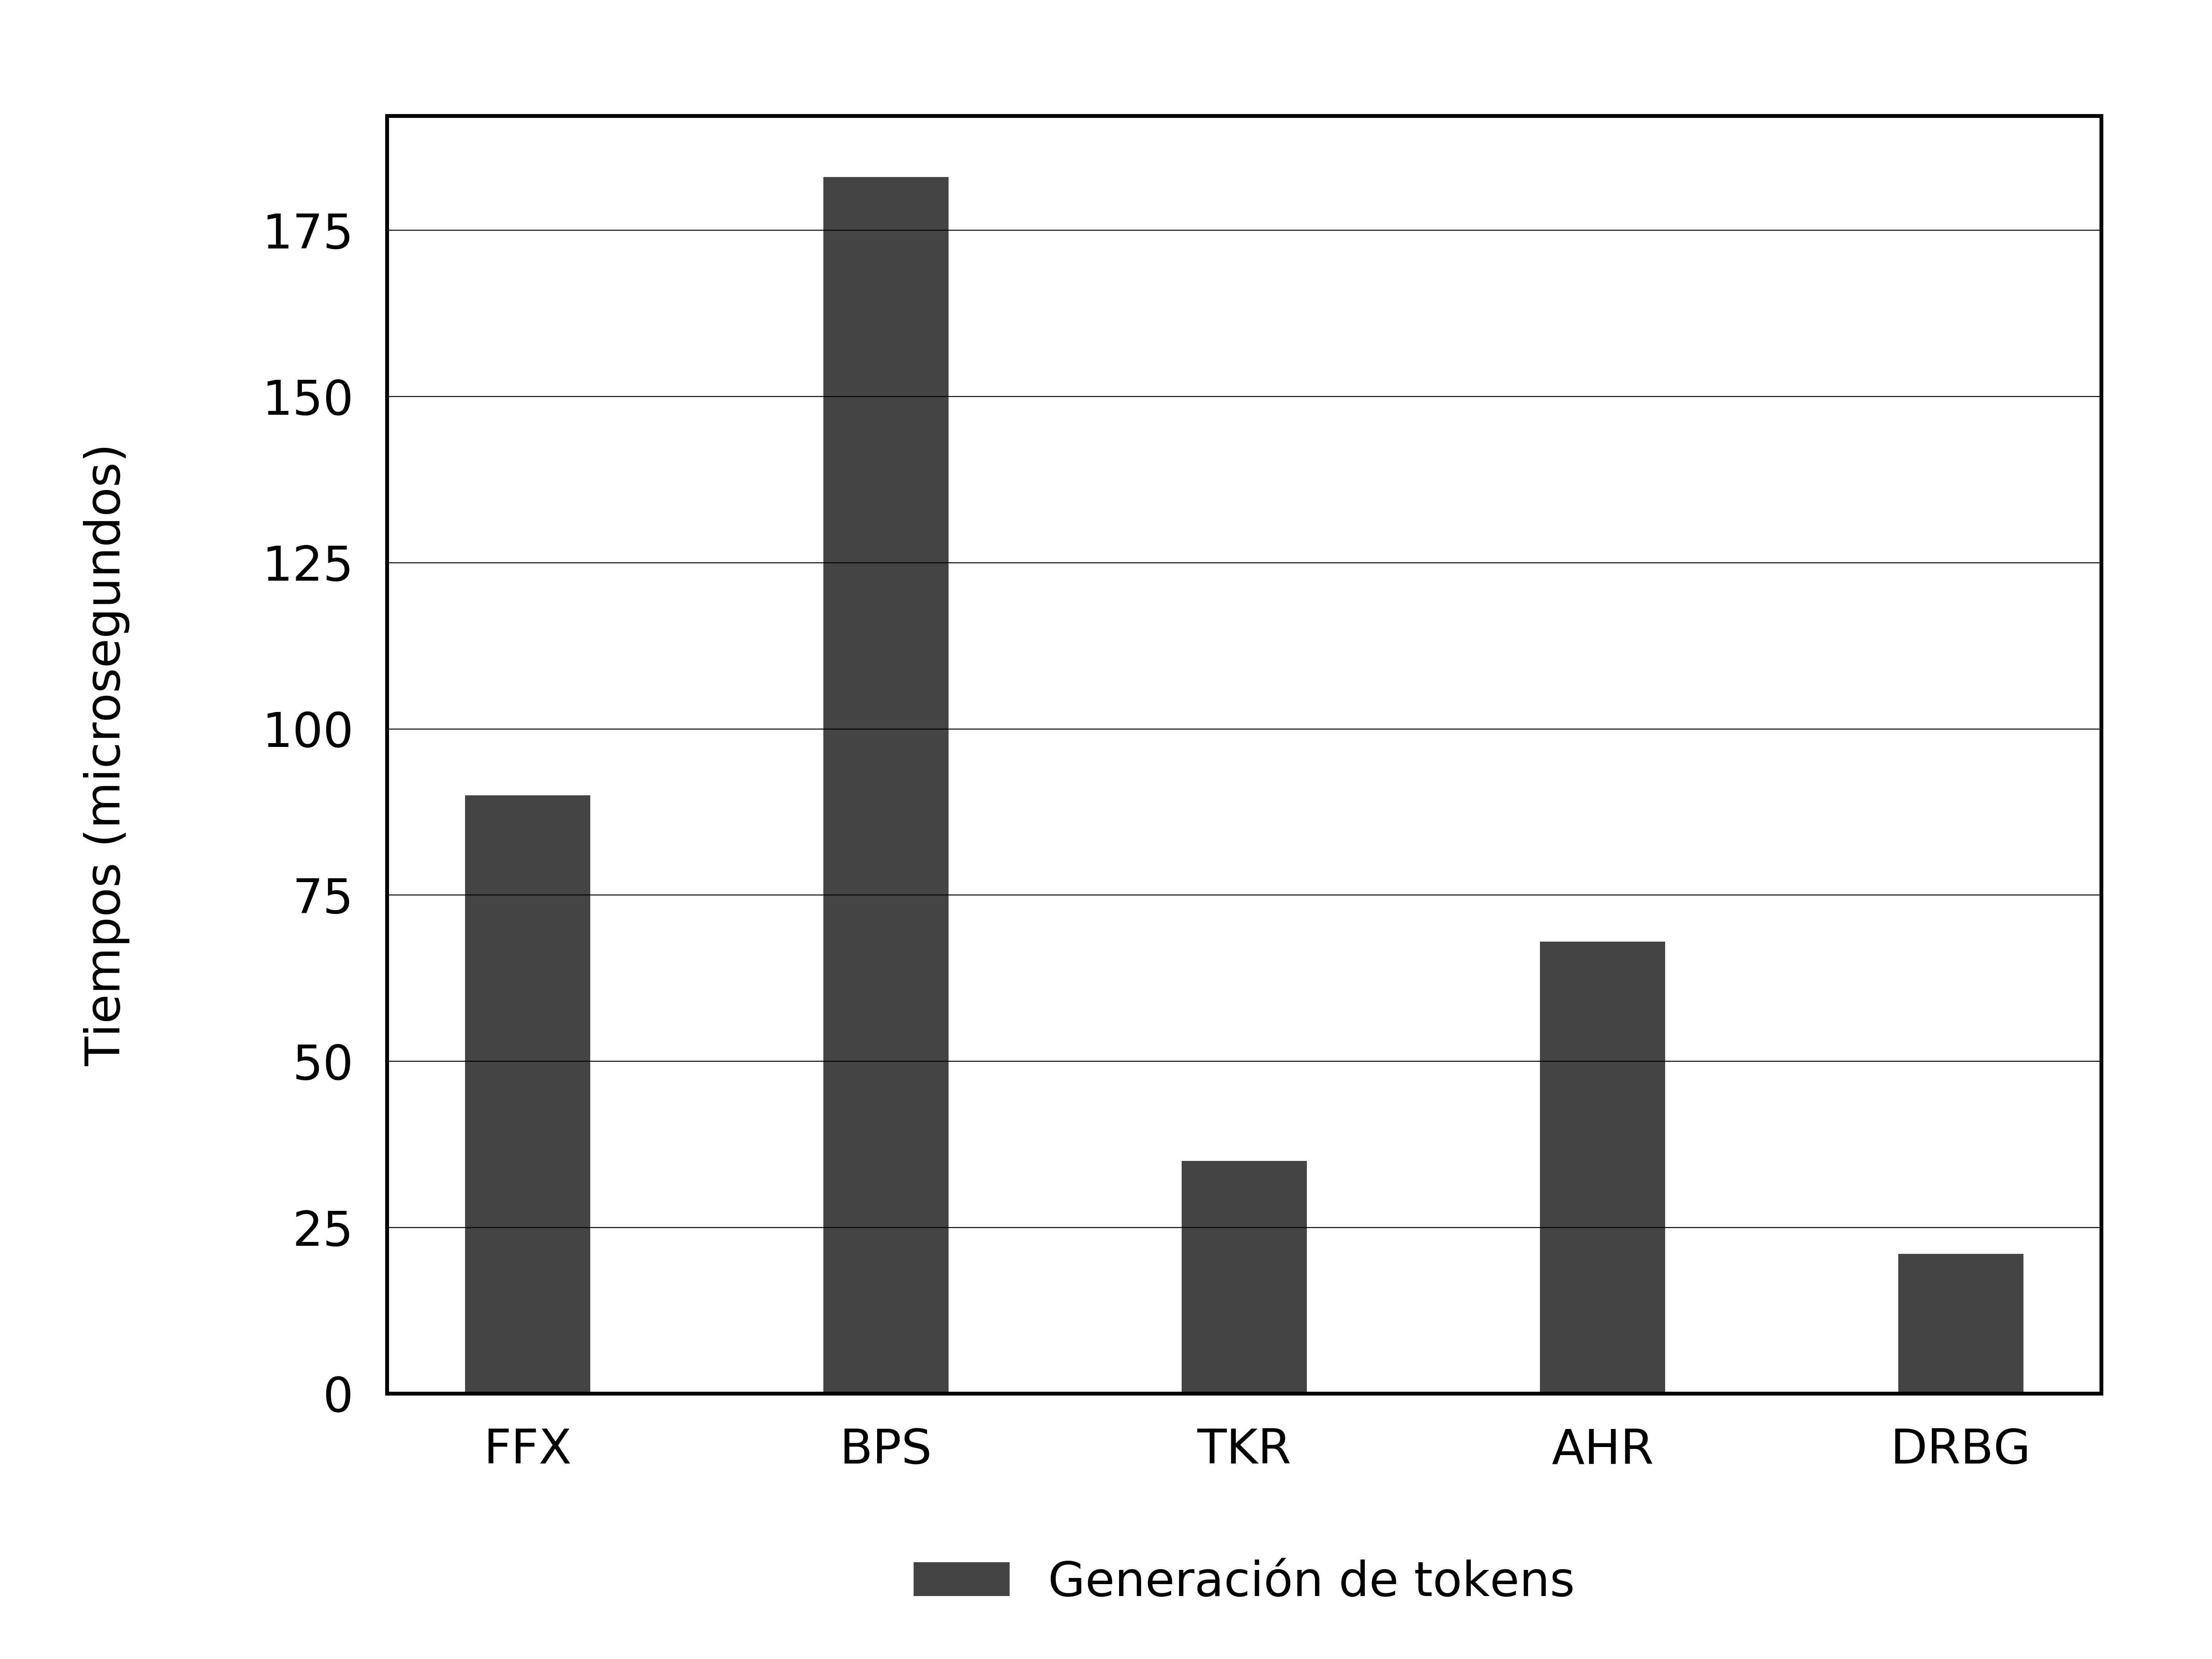
\includegraphics[width=0.5\linewidth]
      {../implementaciones/reportes/tiempos_tokenizacion.png}
    \label{figura:tiempos_tokenizacion}
  }
  \caption{Comparaciones de tiempos.}
  \label{fig_sim}
\end{figure*}


% Resultados

En la Tabla \ref{tabla:tiempos_tokenizacion} y la Figura
\ref{figura:tiempos_unitarios} se muestran los resultados en tiempo de
las ejecuciones de los algoritmos presentados en la Sección
\ref{sec:implementaciones}. Estos se llevaron a cabo en una computadora con las
siguientes características:

\begin{itemize}
  \item \textbf{Procesador:} Intel i5-7200U (2.5 GHz) de 4 núcleos.
  \item \textbf{Sistema operativo:} Arch Linux, kernel 4.17.
  \item \textbf{Base de datos:} MariaDB 10.1.
  \item \textbf{Compilador:} GCC 8.1.1.
\end{itemize}

El procesador ocupado soporta los conjuntos de intrucciones de Intel AES-NI y
RD-SEED \cite{aesni_wp}. Todas los algoritmos tokenizadores que ocupan un
cifrado por bloques usan una implementación de AES con las instrucciones a nivel
de hardware. El DRBG implementado ocupa la instrucción RD-RAND como fuente de
entropía.

% Discusión de resultados

La comparación de los tiempos de tokenización y detokenización muestra como los
algoritmos reversibles son considerablemente más rápidos que los irreversibles.
Este resultado puede resultar un poco contraintuitivo, pues la generación de
tokens reversibles involucra más operaciones; es por esto que en la figura
\ref{figura:tiempos_tokenizacion} se muestran los tiempos de la generación de
tokens solamente, sin tomar en cuenta tiempos de acceso a base de datos.

Además de los tiempos de ejecución, también es importante señalar que los
irreversibles, al operar como funciones de un solo sentido, son más
seguros que los reversibles: un atacante con acceso a la llave de cifrado puede
obtener el número de tarjeta correspondiente si se trata de un método
reversible, mientras que con un método irreversible necesita también acceso a la
base de datos.

% Discusión sobre clasificación

La denominación \textit{no criptográficos}, de la clasificación del PCI SSC
(Sección \ref{sec:clasificacion}), resulta totalmente confusa, pues en
realidad todos los métodos conocidos que caen en esa categoría ocupan
primitivas criptográficas. La segunda categoría (los irreversibles) carece de
utilidad para aplicaciones que procesan pagos con tarjetas de crédito, pues la
habilidad de regresar al número de tarjeta a partir de su token es uno de los
requerimientos principales para los sistemas tokenizadores. Por lo anterior, en
este trabajo se propone una clasificación distinta:

\begin{itemize}
  \item Métodos criptográficos. Todos aquellos que ocupan herramientas
    critográficas.
    \begin{itemize}
      \item Reversibles. Ocupan un esquema de cifrado simétrico: el número
        de tarjeta y una llave entran al mecanismo de tokenización para obtener
        un token; el token y la misma llave entran al mecanismo de
        detokenización para obtener el número de tarjeta original.
      \item Irreversibles. Ocupan herramientas criptográficas para generar el
        token de un número de tarjeta. Ocupan herraminetas externas, como una
        base de datos, para guardar las relaciones entre tokens y números de
        tarjetas.
    \end{itemize}
  \item Métodos no criptográficos. Aquellos posibles métodos que no ocupen
    herramientas relacionadas con la criptografía; por ejemplo, un generador de
    números realmente aleatorio (TRNG, \textit{True Random Number Generator}).
\end{itemize}
